\bgroup
\begin{frame}{Logistic regression classification rule}
The function for classification has the following form:
\begin{equation*}
F(X_i, w) = \sigma(w^T \cdot X_i), \quad \text{where} \quad \sigma(x) = \frac{1}{1+e^{-x}} = \frac{e^{x}}{1+e^{x}}
\end{equation*}
\begin{minipage}{0.45\textwidth}
\begin{itemize}
\onslide<2->{\item $\sigma(x)$ is called \textbf{sigmoid function};}
\onslide<3->{\item $w$ is a vector in $\mathbb{R}^m$, and is called \textbf{weight vector};}
\onslide<4->{\item $w$ is initialized randomly, but will improve as training goes.}
\end{itemize}
\end{minipage}
\onslide<2->{
\begin{minipage}{0.45\textwidth}
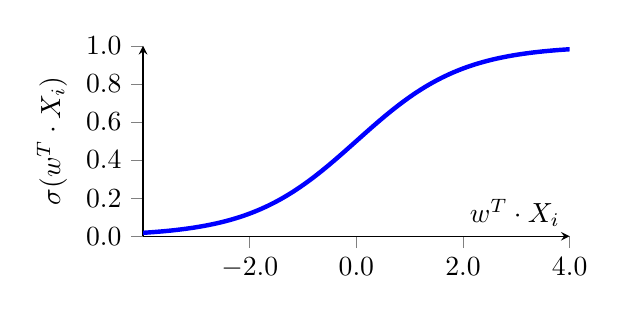
\begin{tikzpicture}
    \begin{axis}[
    	legend pos=north west,
        axis x line=middle,
        axis y line=left,
        x tick label style={/pgf/number format/fixed,
                            /pgf/number format/fixed zerofill,
                            /pgf/number format/precision=1},
        y tick label style={/pgf/number format/fixed,
                            /pgf/number format/fixed zerofill,
                            /pgf/number format/precision=1},
        %grid = major,
        width=7cm,
        height=4cm,
        grid style={dashed, gray!30},
        xmin=-4,     % start the diagram at this x-coordinate
        xmax= 4,    % end   the diagram at this x-coordinate
        ymin= 0,     % start the diagram at this y-coordinate
        ymax= 1,   % end   the diagram at this y-coordinate
        %axis background/.style={fill=white},
        xlabel=$w^T\cdot X_i$,
        ylabel=$\sigma(w^T\cdot X_i)$,
        tick align=outside,
        enlargelimits=false]
      % plot the stirling-formulae
      \addplot[domain=-5:5, blue, ultra thick,samples=500] {1/(1+exp(-x))};
    \end{axis}
\end{tikzpicture}
\end{minipage}
}
\end{frame}
\egroup